%!xelatex = 'xelatex --halt-on-error %O %S'

\documentclass{thuemp}
\begin{document}

% 标题,作者
\emptitle{如何看待毛主席对邓小平的栽培}
\empauthor{江灿}{2019011325}

% 奇数页页眉 % 请在这里写出第一作者以及论文题目
\fancyhead[CO]{{\footnotesize 江灿: 如何看待毛主席对邓小平的栽培}}


%%%%%%%%%%%%%%%%%%%%%%%%%%%%%%%%%%%%%%%%%%%%%%%%%%%%%%%%%%%%%%%%
% 关键词 摘要 首页脚注
%%%%%%%%关键词
\twocolumn[
\begin{@twocolumnfalse}
\maketitle

%%%%%%%%摘要

% \empfirstfoot{2022-04-03}{软件02}{双日下M}{7号}
%%%%%%%%首页角注,依次为实验时间、报告时间、学号、email
\end{@twocolumnfalse}
]
%%%%%%%%!首页角注可能与正文重叠,请通过调整正文中第一页的\enlargethispage{-3.3cm}位置手动校准正文底部位置:
%%%%%%%%%%%%%%%%%%%%%%%%%%%%%%%%%%%%%%%%%%%%%%%%%%%%%%%%%%%%%%%%
%  正文由此开始
\wuhao 
%  分栏开始

\paragraph*{}如何看待毛主席对邓小平的栽培
在1956年9月召开党的八大前夕,毛主席突然提出,建议我们恢复党章当中一个重要的职位——党的总书记
在我们党,我们党最开始的领导人,就是总书记。陈独秀作为我们党的第一个总书记,党的一大一直到五大,做了五届的党书记。但是之后在1945年的党的七大,我们正是修改党章,把总书记这个职务就去掉了。党的领袖明确规定为“中共中央主席”,毛泽东同志在七届一中全会当选为中共国家主席,所以之前,我们国家最高领导人一直是国家主席。但是在当时,毛泽东一方面提出恢复设立总书记这个职位,另一方面又亲自提名邓小平来当。所以在毛主席的支持下,邓小平同志在1956年的党的八大顺利当选了中共中央总书记。
虽然这可能在当时不是很能看出问题的实质,不过在1980年,一个意大利的著名记者,法拉奇,说出:“在西方严重,从50年代起邓小平就是毛泽东的接班人”
在1982年党的十二大修改党章,正式恢复总书记一职,为党内最高领导职务。所以小平在整个人80年代直至逝世,实际上一直是党和国家的最高领导人。
所以说没有毛泽东对小平这个铺垫,所以邓小平后来的成就也很难做到这样。
邓小平三起三落
\paragraph*{}在1934年,小平同志担任中共中央秘书长和中央军委秘书长期间,因为坚决支持毛主席,坚持实事求是,而受到政治上的牵连,被王明路线所迫害,所以这是第一落
第二次落是在文革初期,小平作为刘邓资产阶级司令部“第二号”走资派被打倒。但他在劳动改造的过程中,每天坚持锻炼身体,保持乐观心态,竟然还走出了一个小平小道,成为一个中外人士探求走访的精神圣地。其实上,这也是小平同志设计中国改革开放和现代化建设重要思想的萌芽地。这第二个“落”,直到1973年被任命为国务院的副总理,实际上,是主席是把小平同志保护起来。因为当时在中国,知道未来中国该怎么走的,知道如何去改革开放让刚刚建国不久的新中国走上正轨的,也就只有邓小平了。所以当时毛主席在文革期间,为了避免小平同志被四人帮迫害,让他在一个偏远的地方,能够好好的思考未来中国的道路。这一点,足以看出毛主席的深谋远虑。
最后一次是在1976年4月5日,北京发生了人民观众悼念周总理,批判“四人帮”的五四运动,被“四人帮”诬陷为“中国的匈牙利事件”,向毛主席诬告,把邓小平说成是这个事件的总策划总后台,把中国形容为中国的纳吉(匈牙利总理)。但是这个时候,毛主席却做了一个很深的伏笔,保留了小平同志的党籍。
直到1977年5月9号,邓小平同志第三次复出。
对于这个三起三落的经历,铁娘子对于邓小平的评价是:“有着罕见的忍耐力”。
而我们毛主席对他的评价是:“柔中有刚,绵里藏针;外面和气,内部是钢铁公司”。
正是因为具有这种品格,复出以后的邓小平开始拨乱反正,开辟了一条前无古人之路——中国特色社会主义道路。
在改革开放的伟大实践中,邓小平同志在进一步回答,解决了什么是中国特色社会主义,怎样建成志刚特色社会主义。
邓小平理论主要是:四个一,
围绕一个主题

\paragraph*{}邓小平在逃港问题时,发现对于同一个村庄,在广东的罗芳村,对比香港的罗芳村,一边是每年收入134元,一边是13000元,所以当时的人们都不是不顾一切就要逃港。
所以面临一个问题,什么是社会主义。邓小平使用排除法,贫穷不是社会主义,发展太慢了不是社会主义,平均主义不是社会主义,两极分化不是社会主义,计划经济不是社会主义
法制健全,执行到位。也就是小平同志说的,两个手都要硬。


%%%%%%%%%%%%%%%%%%%%%%%%%%%%%%%%%%%%%%%%%%%%%%%%%%%%%%%%%%%%%%%%

\newpage
% \begin{figure}[H]
% 	\centering
% 	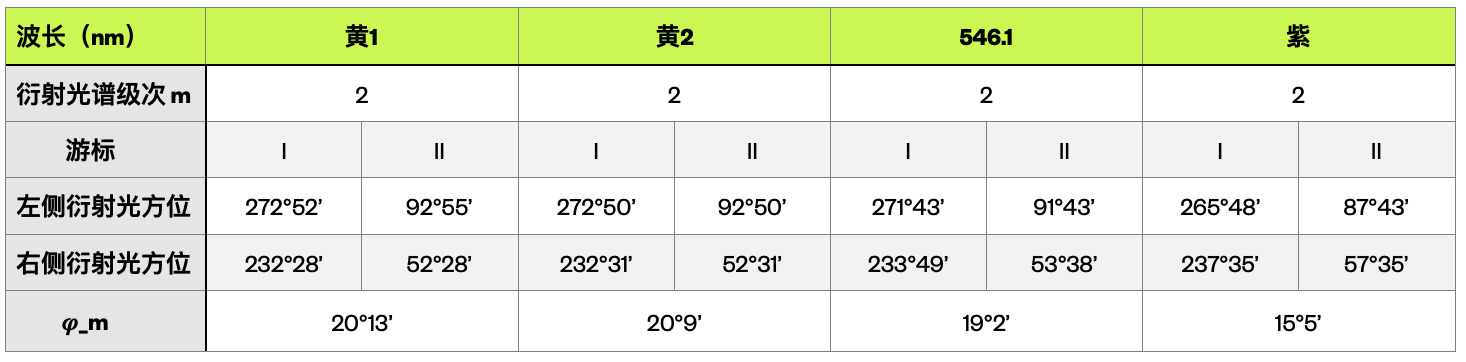
\includegraphics[width=0.8\linewidth]{./image/1.png}
% 	\caption{测定光栅常数和光波波长数据} 
% 	\label{png:1}
% \end{figure}



%%%%%%%%%%%%%%%%%%%%%%%%%%%%%%%%%%%%%%%%%%%%%%%%%%
%  参考文献
%%%%%%%%%%%%%%%%%%%%%%%%%%%%%%%%%%%%%%%%%%%%%%%%%%%%%%%%%%%%%%%%
%  参考文献按GB/T 7714-2015《文后参考文献著录规则》的要求著录. 
%  参考文献在正文中的引用方法:\cite{bib文件条目的第一行}

\renewcommand\refname{\heiti\wuhao\centerline{参考文献}\global\def\refname{参考文献}}
\vskip 12pt

\let\OLDthebibliography\thebibliography
\renewcommand\thebibliography[1]{
  \OLDthebibliography{#1}
  \setlength{\parskip}{0pt}
  \setlength{\itemsep}{0pt plus 0.3ex}
}

{
\renewcommand{\baselinestretch}{0.9}
\liuhao
\bibliographystyle{gbt7714-numerical}
\bibliography{./TempExample}
}


\end{document}
